% \chapter{Experimentální klasifikace pomocí TLS}
% \subsection{TLS příznaky}

% Na základě agregované analýzy Shapleyho hodnot (viz obrázek~\ref{fig:aggregated-shap}) byla identifikována skupina TLS příznaků jako oblast s nejnižším průměrným přínosem (0.046). Tento závěr naznačuje, že příznaky odvozené z TLS certifikátů byly v rámci původního vektorového prostoru podhodnoceny a skýtají potenciál pro další zlepšení klasifikační výkonnosti.

% Nízká váha TLS příznaků ve srovnání s jinými kategoriemi je v kontrastu s výsledky dřívějších prací, například studie Torroleda et al. \cite{torroledo2018hunting}, která prokázala význam TLS certifikátů pro detekci škodlivých domén. Tento nesoulad vedl k rozhodnutí provést cílenou hloubkovou analýzu a rozšíření sady atributů TLS.

% Tabulka~\ref{tab:tls_shap_values} shrnuje příspěvek jednotlivých původně použitých TLS příznaků na základě analýzy metodou SHAP:

% \begin{table}[H]
% \centering
% \caption{Význam vybraných TLS příznaků podle analýzy metodou SHAP.}
% \begin{tabular}{|l|l|}
% \hline
% \textbf{Příznak} & \textbf{SHAP hodnota} \\
% \hline
% \texttt{tls\_root\_cert\_validity\_remaining} & 1.5850 \\
% \texttt{tls\_leaf\_cert\_validity\_len}       & 0.3612 \\
% \texttt{tls\_root\_cert\_validity\_len}       & 0.2098 \\
% \texttt{tls\_leaf\_cert\_validity\_remaining} & 0.1922 \\
% \texttt{tls\_total\_extension\_count}         & 0.1594 \\
% \texttt{tls\_joint\_isoitu\_policy\_crt\_count} & 0.1279 \\
% \texttt{tls\_unique\_SLD\_count}              & 0.1189 \\
% \texttt{tls\_version\_id}                     & 0.1129 \\
% \texttt{tls\_cipher\_id}                      & 0.0774 \\
% \texttt{tls\_CA\_certs\_in\_chain\_ratio}      & 0.0691 \\
% \hline
% \end{tabular}
% \label{tab:tls_shap_values}
% \end{table}

% \subsection{Hloubková analýza TLS příznaků}

% S ohledem na zjištěný potenciál byly identifikovány nové směry pro rozšíření TLS příznaků. Některé relevantní atributy, využívané v jiných studiích, nebyly původně v nástroji \texttt{DomainRadar} implementovány. Vzhledem k jejich prokázanému významu ve světové literatuře bylo rozhodnuto tyto příznaky doplnit a dále zkoumat jejich přínos.

% Pro hlubší analýzu TLS certifikátů byl vyvinut komplexní systém extrakce, který zahrnoval následující charakteristiky:

% \begin{itemize}
%     \item \textbf{Výpočet entropie:} Shannonova entropie textových polí organizace a vydavatele certifikátu, indikující nestandardní nebo syntetické hodnoty.
%     \item \textbf{Hloubka certifikačního řetězce:} Počet certifikátů v řetězci jako indikátor důvěryhodnosti a složitosti infrastruktury.
%     \item \textbf{Analýza politik a rozšíření:} Zjišťování přítomnosti bezpečnostních politik, například podle standardů ISO nebo X.509.
%     \item \textbf{Kombinované ukazatele:} Výpočty poměrů mezi délkami platnosti certifikátů, entropií subjektů a složením certifikačního řetězce.
% \end{itemize}

% \subsubsection{Ukázkový příklad zpracovávaného certifikátu}

% Při analýze jednotlivých certifikátů byly zpracovávány následující části:

% \begin{itemize}
%     \item \textbf{Organizační informace:} Obsah polí Common Name (CN), Organization (O), Country (C) a Location (L).
%     \item \textbf{Platnost certifikátu:} Počáteční (\texttt{notBefore}) a konečné (\texttt{notAfter}) datum.
%     \item \textbf{Rozšíření certifikátu:} Seznam podporovaných rozšíření, například použití pro ověřování serveru (server authentication) nebo klienta (client authentication).
% \end{itemize}

% Cíleným rozšířením a preciznějším zpracováním TLS příznaků je možné lépe využít bezpečnostní charakteristiky certifikátů a zvýšit citlivost detekce škodlivých domén v případech, kdy jiné zdroje informací neposkytují dostatečné odlišující znaky.

% \newpage
% Následující příklad ukazuje strukturu konkrétního TLS certifikátu zpracovaného systémem:
% \begin{lstlisting}[, basicstyle=\ttfamily\small, breaklines=true, numbers=left, frame=single, caption={Struktura TLS certifikátu}, keywordstyle=\bfseries\color{blue}, stringstyle=\color{green!50!black}]
% {
%     "protocol": "TLSv1.3",
%     "cipher": "TLS_AES_256_GCM_SHA384",
%     "count": 4,
%     "certificates": [
%         {
%             "common_name": "E1",
%             "country": "US",
%             "is_root": false,
%             "organization": "Let's Encrypt",
%             "valid_len": 7775999,
%             "validity_start": "2024-04-27 10:25:58",
%             "validity_end": "2024-07-26 10:25:57",
%             "extension_count": 9,
%             "extensions": [
%                 {
%                     "critical": true,
%                     "name": "keyUsage",
%                     "value": "Digital Signature"
%                 },
%                 {
%                     "critical": false,
%                     "name": "extendedKeyUsage",
%                     "value": "TLS Web Server Authentication, 
%                               TLS Web Client Authentication"
%                 },
%                 ...
%                 {
%                     "critical": false,
%                     "name": "ct_precert_scts",
%                     "value": "Signed Certificate Timestamp:\n
%                               Timestamp : Apr 27 11:25:58.305 2024 GMT"
%                 }
%             ]
%         }
%     ]
% }
% \end{lstlisting}

% \subsubsection{Proces analýzy TLS příznaků}
% Pro analýzu byla rozšířena funkce \texttt{analyze\_tls}, která iterativně zpracovává jednotlivé certifikáty v řetězci. Tento proces zahrnoval:
% \begin{enumerate}
%     \item \textbf{Extrakci základních příznaků:} Například hash hodnoty autority, délku platnosti certifikátu a počet rozšíření.
%     \item \textbf{Výpočet složitějších metrik:} Například Shannonova entropie organizace a vydavatele, hloubka řetězce a poměr validních certifikátů.
%     \item \textbf{Detekci anomálií:} Identifikace samo-podepsaných certifikátů s více prvky v řetězci nebo neplatných konfigurací.
% \end{enumerate}

% Výsledky tohoto zpracování jsou částečně založeny na systému vytvořeném A. Horákem, který poskytl základní implementaci analýzy TLS příznaků a přispěl k vytvoření sady nových příznaků.

% \subsubsection{Nově vytvořené TLS příznaky}
% Na základě hloubkové analýzy nezpracovaných dat byla vytvořena rozšířená sada příznaků, které obohacují model o další pohledy na charakteristiky TLS certifikátů. Následující tabulka shrnuje nové příznaky a jejich potenciální přínos pro klasifikaci.

% \begin{table}[H]
% \centering
% \begin{tabular}{|l|p{8cm}|}
% \hline
% \textbf{Nový příznak} & \textbf{Popis a přínos} \\
% \hline
% tls\_cert\_validity\_ratio & Poměr mezi délkou platnosti kořenového a listového certifikátu. Pomáhá identifikovat nestandardní konfigurace certifikátů. \\
% tls\_cert\_validity\_diff & Rozdíl mezi délkou platnosti kořenového a listového certifikátu. Indikátor potenciálně nestandardních vztahů mezi certifikáty v řetězci. \\
% tls\_has\_broken\_or\_expired\_chain & Logický příznak, který označuje, zda je řetězec certifikátů neplatný nebo vypršel. Užitečný pro detekci nesprávné konfigurace. \\
% tls\_is\_self\_signed\_and\_has\_chain & Označuje, zda je certifikát samo-podepsaný, přesto obsahuje více prvků v řetězci. Poukazuje na potenciální anomálie. \\
% tls\_policies\_total\_count & Celkový počet specifických politik v certifikátech. Pomáhá zachytit certifikáty obsahující více politik, což může být běžné u legitimních domén. \\
% tls\_auth\_cert\_ratio & Poměr mezi certifikáty pro autentizaci serveru a klienta. Indikátor neobvyklých konfigurací. \\
% tls\_root\_leaf\_hash\_match & Označuje, zda hash kořenového a listového certifikátu odpovídá. Umožňuje detekci potenciálně zfalšovaných certifikátů. \\
% tls\_chain\_cert\_len\_combined & Kombinace délky řetězce a poměru platnosti certifikátů. Poskytuje komplexní pohled na strukturu certifikačního řetězce. \\
% tls\_cipher\_entropy & Entropie hodnot identifikátorů cipherů v TLS komunikaci. Detekuje vzorce v používaných šifrách. \\
% tls\_version\_entropy & Entropie verzí TLS. Umožňuje detekovat nesoulad nebo nekonzistenci v použitých verzích protokolu. \\
% \hline
% \end{tabular}
% \caption{Nově vytvořené TLS příznaky a jejich přínos.}
% \end{table}

% \subsubsection{Využití příznaků v architektuře sítě}
% \label{new_tls}

% Na základě výše uvedených TLS příznaků byla navržena a natrénována neuronová síť, jejíž architektura je detailně popsána v sekci~\ref{tls_attention}. Síť využívá mechanismus pozornosti, který umožňuje dynamicky identifikovat nejdůležitější příznaky pro danou doménu a tím efektivněji využívat jak stávající, tak nově vytvořené atributy.

% Je však nutné upozornit, že ačkoli architektura využívá pokročilé metody selekce příznaků, není předem zaručeno, že samotné rozšíření TLS příznaků povede ke zlepšení klasifikačního výkonu. Skutečný přínos těchto nových rysů musí být experimentálně ověřen.

% \noindent Navržená architektura přináší následující potenciální výhody:
% \begin{itemize}
%     \item \textbf{Efektivní kombinace příznaků:} Architektura umožňuje propojení původních příznaků s nově odvozenými rysy pro zvýšení klasifikační přesnosti.
%     \item \textbf{Redukce redundantních příznaků:} Mechanismus pozornosti napomáhá identifikaci klíčových atributů a potlačení méně relevantních nebo redundantních informací.
%     \item \textbf{Podpora generalizace:} Dynamická selekce příznaků zlepšuje schopnost modelu přizpůsobit se neznámým doménám a novým útočným vzorům.
% \end{itemize}

% Tento přístup ukazuje, jak lze kombinací pokročilé architektury neuronové sítě a sofistikovaného výběru příznaků cílit na zvýšení robustnosti detekčních systémů.

% Hloubkový rozbor přínosu nově vytvořených příznaků v této architektuře je uveden na obrázku~\ref{fig:tls_classifier_architecture} v kapitole~\ref{chapter:9}.

% \section{Specializovaná neuronová síť} \label{tls_attention}

% Na základě TLS příznaků uvedených v kapitole \ref{chapter:6} byl vytvořen experimentální klasifikátor založený na neuronových sítích. Tento klasifikátor testoval, zda je možné pouze pomocí TLS příznaků efektivně klasifikovat domény, a tím potvrdit jejich význam pro detekci maligních domén. Přístup popsaný v práci Torroleda et al. \cite{torroledo2018hunting} byl využit jako inspirace při návrhu dalších příznaků, které zahrnovaly:
% \begin{itemize}
%     \item Boolovské příznaky, například validaci certifikátu (DV, OV, EV), které indikují úroveň důvěryhodnosti certifikátů.
%     \item Textové příznaky využívající analýzu entropie textových polí certifikátů, což odhaluje nestandardní vzory v textových a organizačních údajích.
%     \item Sociální a organizační příznaky, například identifikace vlastníka certifikátu, které mohou naznačovat opakované vzory v maligních aktivitách.
% \end{itemize}

% Na základě těchto výsledků byla identifikována vysoká přidaná hodnota TLS příznaků, což podporuje jejich další zahrnutí do detekčních mechanismů. Podrobný popis těchto příznaků je uveden v sekci \ref{new_tls}, kde jsou rovněž popsány nové příznaky vytvořené na základě kombinací a transformací původních dat \cite{tlsentropy}. 

% \subsubsection{Architektura TLS klasifikátoru}
% Navržená architektura TLS klasifikátoru byla vytvořena s využitím pokročilých technik neuronových sítí, včetně mechanismu pozornosti (\emph{attention}), který dynamicky identifikuje klíčové příznaky v datech~\cite{vaswani2017attention}. Hlavním cílem tohoto přístupu bylo vytvořit model schopný přesně klasifikovat domény pouze na základě TLS příznaků. Struktura sítě zahrnuje následující prvky:

% \begin{itemize}
%     \item \textbf{Vstupní vrstva}: Síť začíná vstupní vrstvou s 512 neurony, která převádí příznaky do vyšší dimenze. Tato vrstva obsahuje \emph{Batch Normalization} a aktivační funkci \emph{ReLU} pro stabilizaci a zvýšení trénovací efektivity.
%     \item \textbf{První skrytá vrstva}: Obsahuje 256 neuronů, doplněná o normalizaci \emph{Batch Normalization}, \emph{ReLU} aktivační funkci a dropout (\emph{Dropout}) s pravděpodobností 0.3 pro zlepšení generalizace.
%     \item \textbf{Druhá skrytá vrstva}: Tato vrstva obsahuje 128 neuronů, podobně jako předchozí vrstvy zahrnuje \emph{Batch Normalization}, \emph{ReLU} aktivační funkci a dropout.
%     \item \textbf{Skip connection}: Propojení vstupních dat s druhou skrytou vrstvou pomocí \emph{Dense} vrstvy o velikosti 128 neuronů a aktivační funkce \emph{ReLU}. Tento mechanismus slouží jako \emph{residual connection}, který podporuje průchod gradientů a zvyšuje robustnost modelu.
%     \item \textbf{Mechanismus pozornosti}: Klíčovou součástí modelu je pozornost (\emph{attention mechanism}), která přiřazuje váhy jednotlivým příznakům pomocí \emph{Dense} vrstvy s jedním neuronem a aktivační funkcí \emph{sigmoid}. Tyto váhy se následně aplikují na vstupní data.
%     \item \textbf{Výstupní vrstva}: Síť končí jedním neuronem s aktivační funkcí \emph{sigmoid}, který produkuje pravděpodobnostní skóre pro binární klasifikaci.
% \end{itemize}

% Tato architektura byla implementována v knihovně Keras a její struktura je vizualizována na obrázku \ref{fig:tls_classifier_architecture}. Obrázek ukazuje logický tok dat, včetně implementace upraveného mechanismu pozornosti (attention).

% \begin{figure}[H]
%     \centering
%     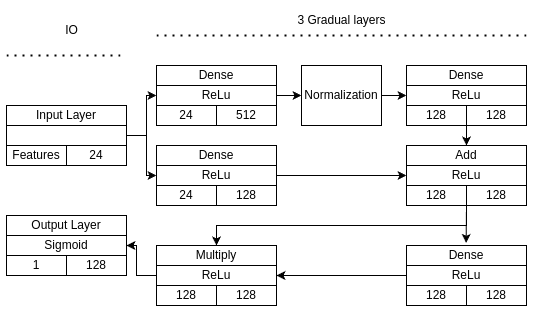
\includegraphics[width=0.8\textwidth]{obrazky-figures/tls_attention.png}
%     \caption{Architektura TLS klasifikátoru.}
%     \label{fig:tls_classifier_architecture}
% \end{figure}











% \section{Specializovaný TLS model (Attention-based)}\label{res:attention_tls}

% Specializovaný model založený výhradně na TLS příznacích byl navržen s cílem ověřit, zda lze z vlastností TLS handshake a certifikátů domén efektivně detekovat škodlivé aktivity. Architektura využívá jednoduchý mechanismus pozornosti (attention), který dynamicky váží vstupní příznaky a zvýrazňuje ty nejdůležitější. Následně jsou tyto zpracované reprezentace předány skrze hlubší síť s \texttt{skip connection}, která umožňuje modelu lépe zachytit komplexní vztahy mezi příznaky.

% Výhodou tohoto přístupu je jeho úzké zaměření na omezený počet (24) vysoce specifických TLS atributů, které nevyžadují zpracování textového obsahu ani analýzu chování domény. Díky tomu je model lehký, rychlý a snadno implementovatelný i v prostředích s omezenými výpočetními prostředky.

% \subsection{Výsledky klasifikace}

% Model byl testován ve třetí klasifikační fázi samostatně pro phishingové a malware domény. Tabulka~\ref{tab:attention_tls_results} shrnuje dosažené metriky pro obě úlohy.

% \begin{table}[H]
% \centering
% \begin{tabular}{|l|c|c|}
% \hline
% \textbf{Metrika} & \textbf{Phishing} & \textbf{Malware} \\
% \hline
% Přesnost (Accuracy)     & \texttt{0.9934 ± 1.4e-04} & \texttt{0.9896 ± 7.8e-05} \\
% Precision (Přesnost)    & \texttt{0.9882 ± 8.8e-05} & \texttt{0.9660 ± 7.2e-05} \\
% Recall (Úplnost)        & \texttt{0.9722 ± 5.2e-05} & \texttt{0.9383 ± 5.7e-05} \\
% F1 Skóre                & \texttt{0.9801 ± 6.4e-05} & \texttt{0.9519 ± 4.8e-05} \\
% ROC AUC                 & \texttt{0.9849 ± 7.9e-05} & \texttt{0.9671 ± 6.1e-05} \\
% \hline
% \end{tabular}
% \caption{Výsledky klasifikace modelu \texttt{attention\_tls} ve fázi~3 pro phishing a malware domény (v1.1, 10 běhů)}
% \label{tab:attention_tls_results}
% \end{table}

% Z tabulky je patrné, že i čistě technické příznaky získané z TLS spojení poskytují dostatečné množství informací pro úspěšnou detekci škodlivých domén. Model dosahuje vysoké přesnosti a F1 skóre, a to jak v případě phishingu, tak i malware domén. Phishingové domény jsou detekovány s mírně vyšší úspěšností, avšak i výkon na malware datech zůstává velmi dobrý a překonává většinu běžných baseline metod.

% \subsection{Analýza matic záměn}

% Model \texttt{attention\_tls} dosahuje velmi dobrého poměru mezi citlivostí a přesností. Matice záměn na obrázcích~\ref{fig:attention_tls_conf_matrix_phishing} a~\ref{fig:attention_tls_conf_matrix_malware} ukazují nízký počet falešných pozitivních i falešných negativních vzorků.

% \begin{figure}[H]
%     \centering
%     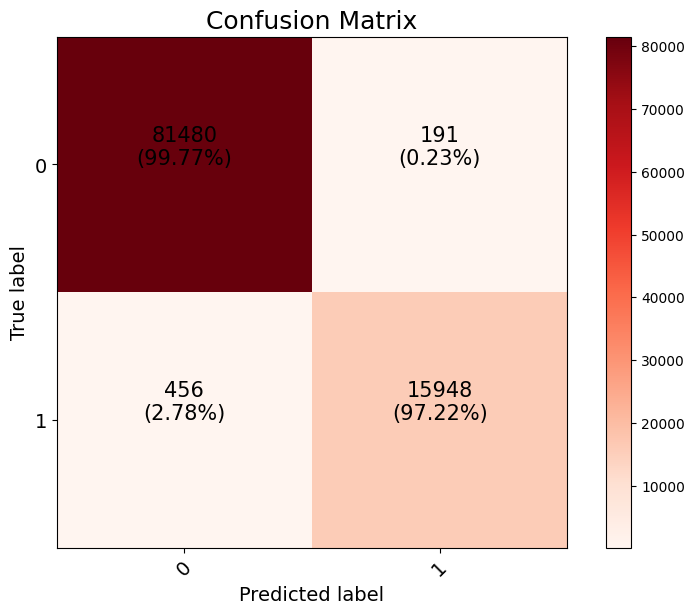
\includegraphics[width=0.8\textwidth]{obrazky-figures/attention_tls_stage_3_phishing_v1.1_confusion_matrix.png}
%     \caption{Matice záměn modelu \texttt{attention\_tls} pro phishingové domény (fáze~3)}
%     \label{fig:attention_tls_conf_matrix_phishing}
% \end{figure}

% \begin{figure}[h!]
%     \centering
%     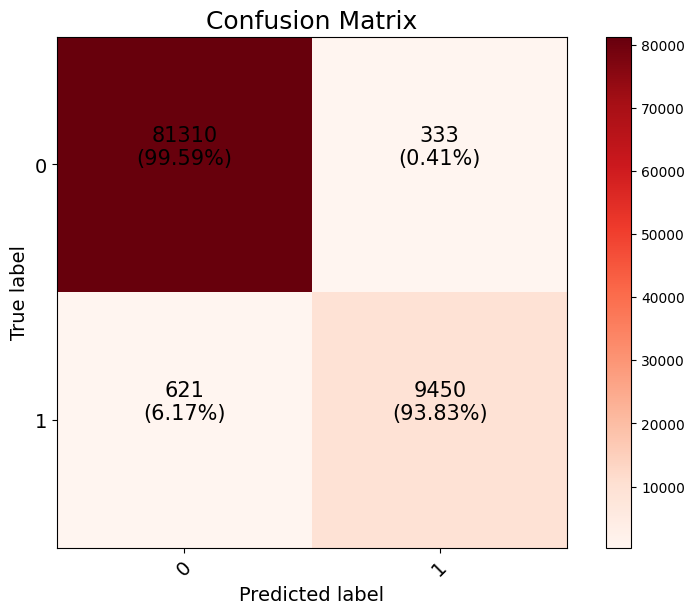
\includegraphics[width=0.8\textwidth]{obrazky-figures/attention_tls_stage_3_malware_v1.1_confusion_matrix.png}
%     \caption{Matice záměn modelu \texttt{attention\_tls} pro malware domény (fáze~3)}
%     \label{fig:attention_tls_conf_matrix_malware}
% \end{figure}

% \subsection{Shrnutí výkonu modelu}

% Model \texttt{attention\_tls} ukazuje, že i bez přístupu k obsahu domény nebo DNS informacím lze dosáhnout velmi kvalitní detekce škodlivých domén pouze na základě TLS metadat. Mezi hlavní výhody modelu patří:

% \begin{itemize}
%     \item Vysoká přesnost a robustnost při klasifikaci phishingových i malware domén.
%     \item Nízká falešná pozitivita, což je důležité pro praktické nasazení.
%     \item Architektura s pozorností a \texttt{skip connection} zvyšuje schopnost modelu adaptovat se na různé struktury dat.
%     \item Nízké nároky na vstupní data a výpočetní prostředky – vhodné pro edge nasazení i systémy bez přístupu k aplikační vrstvě.
% \end{itemize}

% Celkově lze model \texttt{attention\_tls} považovat za vysoce efektivní komponentu klasifikační pipeline, která umožňuje rozšířit detekční pokrytí i na situace, kdy jsou dostupná pouze transportní metadata.

% \section{Výsledky finální pipeline.}
% \begin{sidewaystable}
% \centering
% \small
% \resizebox{\textwidth}{!}{%
% \begin{tabular}{|l|cc|cc|cc|}
% \hline
% \textbf{Metrika} & \multicolumn{2}{c|}{\textbf{Stage 1}} & \multicolumn{2}{c|}{\textbf{Stage 2}} & \multicolumn{2}{c|}{\textbf{Stage 3}} \\
% \cline{2-7}
%  & \textbf{Phishing} & \textbf{Malware} & \textbf{Phishing} & \textbf{Malware} & \textbf{Phishing} & \textbf{Malware} \\
% \hline
% Accuracy           & \texttt{0.9721 ± 1.2e-04} & \texttt{0.9702 ± 1.1e-04} & \texttt{0.9910 ± 9.6e-05} & \texttt{0.9902 ± 9.2e-05} & \texttt{0.9963 ± 9.2e-05} & \texttt{0.9921 ± 1.1e-04} \\
% Precision          & \texttt{0.8962 ± 9.5e-05} & \texttt{0.9025 ± 9.0e-05} & \texttt{0.9628 ± 8.2e-05} & \texttt{0.9575 ± 7.9e-05} & \texttt{0.9959 ± 2.1e-07} & \texttt{0.9834 ± 2.4e-07} \\
% Recall             & \texttt{0.9144 ± 1.0e-04} & \texttt{0.9187 ± 9.5e-05} & \texttt{0.9790 ± 8.9e-05} & \texttt{0.9704 ± 8.0e-05} & \texttt{0.9791 ± 2.5e-07} & \texttt{0.9617 ± 2.8e-07} \\
% F1 Score           & \texttt{0.9051 ± 9.2e-05} & \texttt{0.9105 ± 8.8e-05} & \texttt{0.9708 ± 7.4e-05} & \texttt{0.9639 ± 6.6e-05} & \texttt{0.9875 ± 1.8e-07} & \texttt{0.9722 ± 2.1e-07} \\
% ROC AUC            & \texttt{0.9874 ± 7.8e-05} & \texttt{0.9889 ± 7.0e-05} & \texttt{0.9990 ± 4.3e-06} & \texttt{0.9973 ± 4.0e-06} & \texttt{0.9997 ± 2.4e-06} & \texttt{0.9990 ± 4.7e-06} \\
% \hline
% \end{tabular}%
% }
% \caption{Výsledky klasifikace phishingových a malware domén napříč jednotlivými fázemi – validační sada}
% \label{tab:final_pipeline_all_stages_rotated}
% \end{sidewaystable}



% \begin{sidewaystable}
% \centering
% \small
% \resizebox{\textwidth}{!}{%
% \begin{tabular}{|l|cc|cc|cc|}
% \hline
% \textbf{Metrika} & \multicolumn{2}{c|}{\textbf{Stage 1}} & \multicolumn{2}{c|}{\textbf{Stage 2}} & \multicolumn{2}{c|}{\textbf{Stage 3}} \\
% \cline{2-7}
%  & \textbf{Phishing} & \textbf{Malware} & \textbf{Phishing} & \textbf{Malware} & \textbf{Phishing} & \textbf{Malware} \\
% \hline
% Accuracy           & \texttt{0.9673} & \texttt{0.9625} & \texttt{0.9851} & \texttt{0.9762} & \texttt{0.9892} & \texttt{0.9784} \\
% Precision          & \texttt{0.8841} & \texttt{0.8906} & \texttt{0.9508} & \texttt{0.9450} & \texttt{0.9900} & \texttt{0.9840} \\
% Recall             & \texttt{0.9027} & \texttt{0.8974} & \texttt{0.9675} & \texttt{0.9563} & \texttt{0.9481} & \texttt{0.9150} \\
% F1 Score           & \texttt{0.8933} & \texttt{0.8939} & \texttt{0.9591} & \texttt{0.9506} & \texttt{0.9536} & \texttt{0.9413} \\
% ROC AUC            & \texttt{0.9812} & \texttt{0.9785} & \texttt{0.9965} & \texttt{0.9932} & \texttt{0.9916} & \texttt{0.9710} \\
% \hline
% \end{tabular}%
% }
% \caption{Výsledky klasifikace phishingových a malware domén napříč jednotlivými fázemi – verifikační sada}
% \label{tab:final_pipeline_all_stages_ver}
% \end{sidewaystable}
